\chapter{Электрическое поле в диэлектриках}

\section{Поляризация диэлектриков}

    \begin{definition}
        \textbf{Диэлектрики} -- это вещества, которые не имеют свободных
        зарядов, то есть таких зарядов, которые могли бы перемещаться по всему
        объёму тела. Заряды в них могут смещаться лишь на расстояния порядка
        межатомных.
    \end{definition}
    
    Однако, при помещении диэлектрика в электрическое поле он начинает
    взаимодействовать с ним:
    
    \begin{enumerate}
        \item заметно искажение поле;
        \item диэлектрик приобретает заметный макроскопический момент, из-за
            которого он начинает взаимодействовать с полем: ориентируется и
            втягивается в область более сильного поля
            \[
                F = p\frac{\partial E}{\partial x}; \ p = ql \ne 0
            \]        
    \end{enumerate}
    
    \begin{definition}
    Разделение зарядов в диэлектрике и появление у него дипольного момента при
    помещении во внешнее электрическое поле \( \vec{E} \) называется
    \textbf{поляризацией} диэлектрика во внешнем электрическом поле
    \( \vec{E} \).
    \end{definition}
    
    В зависимости от структуры и химического состава возможны несколько
    механизмов поляризации диэлектрика.
    
\section{Механизмы поляризации}

\subsection{Электронная поляризация}
    По этому механизму поляризуются диэлектрики, молекулы которых не имеют
    собственного дипольного момента (\( p_i = 0 \)), например,
    \( H_2, O_2, CH_4, CO_2 \).
    
    Однако, при их помещении в поле \( \vec{E} \) электронная оболочка слегка
    деформируется и каждая молекула приобретает дипольный момент, и,
    следовательно, весь диэлектрик приобретает дипольный момент.
    
\subsection{Ориентационная поляризация}

    Этот механизм наблюдается у веществ, молекулы которых имеют собственный
    дипольный момент (\( p_i \ne 0 \)), таких как \( H_2O \text{ и } NH_3\).
    В отсутствие внешнего поля, все эти элементарные диполи ориентированы
    хаотично, и образец в целом нейтрален. Но при наложении поля элементарные
    диполи \textit{слегка} выстраиваются вдоль линий поля.
    
\subsection{Ионная поляризация}

    Этот механизм наблюдается у ионных кристаллов. Рассмотрим его на примере
    \( Na^{+}Cl^{-} \). В отсутствие внешнего поля решётки \( Na^{+} \) и
    \( Cl^{-} \) располагаются так, что кристалл нейтрален. При наложении поля,
    решётки \textit{немного} смещаются и, в результате, кристалл поляризуется.
    
\subsection{Механическая поляризация (пьезоэлектрический эффект)}

    Механизм наблюдается у кристаллов, не имеющих центра симметрии, например,
    \( BaTiO_3 \). При этом меанизме поляризации кристалл поляризуется под
    воздействием внешних механических напряжений.
      
\section{Поверхностные и объёмные связанные заряды}

    При поляризации однородного диэлектрика поляризационные, или
    \textbf{связанные}, заряды выделяются только на его поверхности.
    Однако, разделить их нельзя, так как получится два поляризованных образца.
    Если же диэлектрик неоднороден, то при помещении его во внешнее поле
    \( \vec{E} \), в нем появляются не только поверхностные, но и объёмные
    связанные заряды.
    \begin{figure}[b!]
        \center
        \subfigure[Однородный диэлектрик]{
            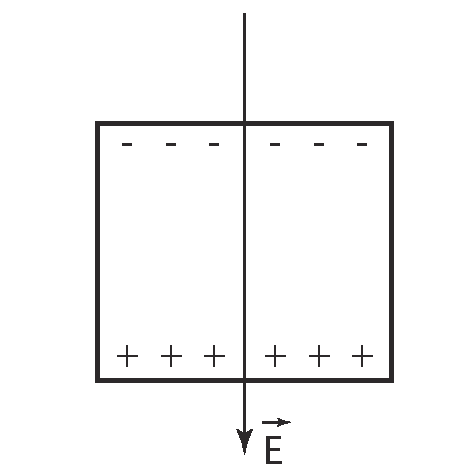
\includegraphics[width=0.47\textwidth]{lec05/homogeneous.pdf}
        }
        \hfill
        \subfigure[Неоднородный диэлектрик]{
            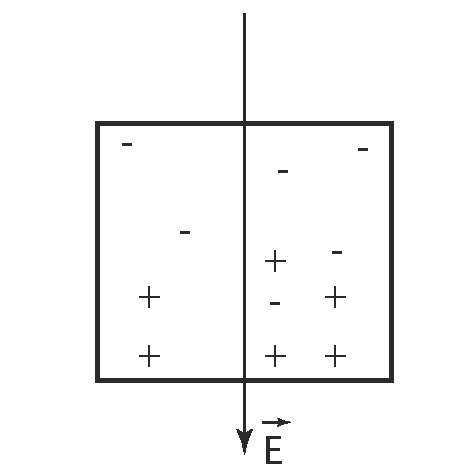
\includegraphics[width=0.47\textwidth]{lec05/inhomogeneous.pdf}
        }
        \caption{Связанные заряды в диэлектриках}
    \end{figure}
\section{Поляризованность}
    
    Количественной характеристикой степени поляризации диэлектрика является его
    \textbf{поляризованность}.
    
    \begin{definition}
        \textbf{Поляризованность} \( \vec{P} \) -- это дипольный момент единицы
        объёма диэлектрика.
    \end{definition}
    \begin{equation}
        \vec{P} = \frac{\sum \vec{p_i}}{\Delta V} = n \midnum{\vec{p_i}},
    \end{equation}
    где \( \vec{P} \) -- вектор поляризованности, \( \vec{p_i} \) -- дипольный
    момент \( i \)-молекулы,
    \( \midnum{\vec{p_i}} = \frac{\sum \vec{p_i}}{N} \) -- средний дипольный
    момент одной молекулы, \( n = \frac{N}{\Delta V} \) -- концентрация молекул,
    \( N \) -- количество молекул в единице объёма.
    
    Если поляризация \textbf{однородная}, то есть однороден поляризованный
    диэлектрик, то поверхностную плотность \( \sigma' \) связанного
    поверхностного заряда можно легко связать с вектором поляризованности
    \( \vec{P} \). Для этого вырежем из диэлектрика косую призму и определим её
    дипольный момент:
    \[
        p = q' l = \sigma' Sl
    \]
    Объем призмы:
    \[
        V = lS_{\perp} = lS\cos\alpha
    \]
    
    Тогда, по определению:
    \[
        P = \frac{p}{V} = \frac{\sigma'}{\cos\alpha}
    \]
    Или:
    \begin{equation}
        \sigma' = P\cos\alpha = P_n,
    \end{equation}
    где \( P_n \) -- нормальная компонента вектора \( \vec{P} \).
    
    Если поляризация неоднородная, то, в общем случае, для него справедлива
    теорема Гаусса для поля вектора \( \vec{P} \):
    \begin{theorem}
        Поток вектора \( \vec{P} \) через произвольную замкнутую поверхность
        \( S \) равен суммарному связанному заряду \( q_S' \), охваченному
        поверхностью \( S \).
        \begin{equation}
            \oiint\limits_S \vec{P}\cdot\vec{dS} = -q_S' \label{eq5:X3n1}
        \end{equation}
    \end{theorem}
    
    
    Если заряд \( q' \) распределён по образцу непрерывно, то
    \[
        q_S' = \iiint\limits_V \rho' dV.
    \]
    А так как по теореме Остроградского
    \[
        \oiint\limits_S \vec{P}\cdot\vec{dS} = \iiint\limits_V \div\vec{P}dV,
    \]
    то, в силу произвольности \( S \) и \( V \):
    \begin{equation}
        \rho' = -\div\vec{P} \label{eq5:X3n2}
    \end{equation}
    Уравнение (\ref{eq5:X3n2}) -- это дифференциальная форма теоремы Гаусса для
    вектора \( \vec{P} \).
    
\section{Электрическое поле в диэлектриках}
    
    \begin{figure}[b!]
        \center
        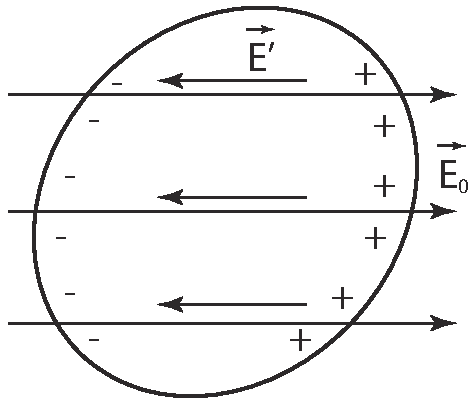
\includegraphics[width=0.47\textwidth]{lec05/E_and_isolator.pdf}
        \caption{Электрическое поле в диэлектриках}
    \end{figure}

    Появление индуцированных связанных зарядов в образце при его помещении во
    внешнее поле \( \vec{E_0} \) порождает индуцированное поле \( \vec{E'} \),
    которое, складываясь с \( \vec{E_0} \), и даёт результирующее внешнее поле
    \( \vec{E} \):
    \begin{equation}
        \vec{E} = \vec{E_0} + \vec{E'}
    \end{equation}
    % еще есть много надписей, видимо относящихся к картинке:
    %  \( \Delta\varphi = 0 \) или \( \Delta\varphi = -\frac{\rho}{\eps_0} \) для нахождения результирующего поля \( \vec{E} \), так как заряды создают поле \( \vec{E} \) и конфигурируются им.

\section{Вектор \textbf{D}}

    Так как поле \( \vec{E} \) создаётся всеми зарядами: и свободными \( q \),
    и связанными \( q' \), то теорема Гаусса для поля \( \vec{E} \) будет
    выглядеть так:
    \begin{equation}
        \oiint\limits_S \vec{E}\cdot\vec{dS} = \frac{1}{\eps_0}(q+q')_S
        \label{eq5:1}
    \end{equation}
    
    Чтобы избавиться от неизмеряемого заряда \( q_S' \) применим теорему Гаусса для поля \( \vec{P} \) и тогда (\ref{eq5:1}):
    \[
        \oiint\limits_S (\eps_0\vec{E} + \vec{P})\cdot\vec{dS} = q_S
    \]
    
    Обозначим комбинацию в скобках за \( \vec{D} \):
    \begin{equation}
        \vec{D} = \eps_0\vec{E} + \vec{P} \label{eq5:2}
    \end{equation}
    
    Тогда теорема Гаусса для поля \( \vec{D} \):
    \begin{equation}
        \oiint\limits_S \vec{D}\cdot\vec{\dd S} = q_S
        \label{eq5:3}
    \end{equation}
    
    При непрерывном распределении заряда
    \[
        q_S = \iiint\limits_V \rho \dd V.
    \]
    Тогда, по теореме Остроградского:
    \[
        \oiint\limits_S \vec{D}\cdot\vec{dS} = \iiint\limits_V \div\vec{D}\dd V 
    \]
    
    В силу произвольности \( S \) и \( V \):
    \begin{equation}
        \div\vec{D} = \rho \label{eq5:4}
    \end{equation}
    
    Уравнение (\ref{eq5:4}) -- дифференциальная форма теоремы Гаусса для поля
    \( \vec{D} \). Таким образом, источником поля \( \vec{D} \) являются только
    свободные (избыточные), заряды, а поля \( \vec{E} \) -- и избыточные,
    и связанные.
     
\section{Связь между векторами \textbf{P}, \textbf{E} и \textbf{D}}

    Так как обычные (\( E \ll E_{\textit{межатом}} \sim
    10^{11} \text{В}/\text{м} \)) поля вызывают слабую деформацию
    электронных оболочек, то можно считать, что \( P \sim E \), а так как по
    размерности \( [P] = [\eps_0E] \) и
    \( \vec{P} \uparrow\uparrow \vec{E} \) в изотропных диэлектриках, то можно
    считать, что
    \begin{equation}
        \vec{P} = \varkappa\eps_0\vec{E} \label{eq5:5}
    \end{equation}
    
    Безразмерный множитель \( \varkappa \) в (\ref{eq5:5}) называетс
    \textbf{диэлектрической восприимчивостью} диэлектрика.
    
    Подставив (\ref{eq5:5}) в (\ref{eq5:2}), получаем:
    \begin{equation}
        \vec{D} = \eps_0\vec{E}(\varkappa+1) =
        \eps\eps_0\vec{E}
        \label{eq5:6}
    \end{equation}
    
    Скалярный множитель \( \eps \) называется
    \textbf{диэлектрической проницаемостью} вещества. Обычно, для диэлектриков
    \( \eps \sim 1\ldots3\):
    \begin{itemize}
        \item для вакуума: \( \eps = 1 \),
        \item для воздуха: \( \eps = 1.0006 \),
        \item для стекла: \( \eps \sim 1.5 \),
        \item но для воды: \( \eps = 81 \).
    \end{itemize}
    
    Формулы (\ref{eq5:2}), (\ref{eq5:5}) и (\ref{eq5:6}) выражают искомую связь
    между векторами \( \vec{P}, \vec{E} \) и \( \vec{D} \).
    
\section{Конденсатор с диэлектриком}

    Ёмкость конденсатора с диэлектриком будет увеличена, так как связанные
    заряды уменьшают поле \( \vec{E} \), следовательно, уменьшается  напряжение
    \( U \), следовательно увеличивается \( C \), так как
    \( C\uparrow = \frac{q=\const}{U\downarrow} \).
    \begin{figure}[h]
        \center
        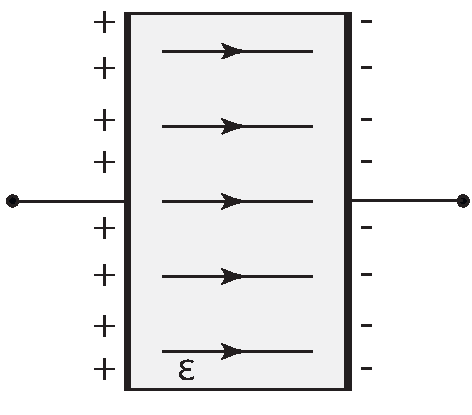
\includegraphics[width=0.47\textwidth]{lec05/capacitor.pdf}
        \caption{Конденсатор с диэлектриком}
    \end{figure}
    Вычислим ёмкость конденсатора, заполненного диэлектриком с диэлектрической
    проницаемостью \( \eps \). Для пустого плоского конденсатора
    \[
        C_0 = \frac{\eps_0S}{d}.
    \]
    Пусть в нем находится диэлектрик \( \eps \). Охватим участок верхней
    пластины замкнутым цилиндром
    \( S_{\textit{цил}} = S_{\textit{бок}} + 2S_{\textit{тор}} \).
    
    Так как вне конденсатора \( E = 0 \) и \( D = 0 \), то, по теореме Гаусса:
    \[
        \underbrace{\oiint\limits_{ S_{\textit{цил}} }\vec{D}\cdot\vec{dS}
        }_{DS_{\textit{тор}}} = q_S = \sigma S_{\textit{тор}}
    \]
    
    Тогда \( \sigma = D \), где \( \sigma \) -- поверхностная плотность
    свободных зарядов. И тогда
    \[
        C = \frac{q}{U} = \frac{\sigma S}{Ed} = \frac{DS}{Ed} =
        \frac{\eps\eps_0 S}{d} = \eps C_0
    \]
    
    Таким образом, ёмкость конденсатора с диэлектриком в \( \eps \) раз
    больше, чем ёмкость пустого конденсатора.
    
\section{Распределение энергии в электрическом поле}

    Запишем энергию плоского конденсатора с диэлектриком:
    \[
        W = \frac{CU^2}{2} = \frac{\eps\eps_0E^2Sd}{2} =
        \frac{\eps\eps_0E^2}{2}V_E,
    \]
    где \( V_E \) -- объем, занимаемый полем \( \vec{E} \). Таким образом,
    \( W \sim V_E \). Можно предположить, что энергия локализована в поле
    \( \vec{E} \).
    
    Тогда объёмная плотность энергии электрического поля:
    \[
        w_E = \frac{W}{V_E} = \frac{\eps\eps_0E^2}{2} =
        \frac{ED}{2} \left(\frac{\text{Дж}}{\text{м}^3}\right)
    \]
    
\section{Граничные условия}

    Пусть два диэлектрика \( \eps_1 \) и \( \eps_2 \) с общей
    границей их раздела помещены во внешнее поле \( \vec{E_0} \). Линии поля
    \( \vec{E_0} \) на границе раздела будут испытывать преломление, так как
    на границе появятся заряды \( \pm \sigma' \).
    
    Установим характер преломления линий поля \( \vec{E} \) и \( \vec{D} \):
    \begin{enumerate}
        \item Теорема Гаусса для поля \( \vec{D} \).
        
        Охватим малый участок на границе раздела замкнутым цилиндром
        \( S_{\textit{цил}} = S_{\textit{бок}} + 2S_{\textit{тор}} \).
        
        \[
            \oiint\limits_{S_{\textit{цил}}} \vec{D}\cdot\vec{dS} =
            q_{\textit{своб}} = 0,
        \]
        так как в диэлектриках свободных зарядов нет. Следовательно:
        \[
            -D_{n1}S_{\textit{тор}}^{\text{верх}} + 
            D_{n2}S_{\textit{тор}}^{\text{ниж}} = 0,
        \]
        \begin{equation}
            D_{n2} = D_{n1}
            \label{eq5:n1}
        \end{equation}
        
        Уравнение (\ref{eq5:n1}) означает, что нормальная компонента вектора
        \( \vec{D} \) на границе раздела непрерывна.
        
        \item Теорема о циркуляции поля \( \vec{E} \).
        
        Охватим малый участок границы раздела узким контуром \( C \):
        \[
            \oint\limits_C \vec{E}\cdot\vec{dl} = 0,
        \]
        отсюда следует, что при \( h \ll l \):
        \[
            E_{\tau1}l_{\textit{верх}} - E_{\tau2}l_{\textit{ниж}} = 0,
        \]
        \begin{equation}
            E_{\tau2} = E_{\tau1}
            \label{eq5:n2}
        \end{equation}
        
        Уравнение (\ref{eq5:n2}) означает, что касательная компонента вектора
        \( \vec{E} \) на границе раздела непрерывна.
    \end{enumerate}
    
    Если в (\ref{eq5:n1}) и (\ref{eq5:n2}) подставить связь \( \vec{D} \) и
    \( \vec{E} \), то:
    \begin{align*}
        & \frac{E_{n2}}{E_{n1}} = \frac{\eps_1}{\eps_2}, \\
        & \frac{D_{\tau2}}{D_{\tau1}} = \frac{\eps_1}{\eps_2},
    \end{align*}
    то есть происходит разрыв нормальной компоненты вектора \( \vec{E} \) и
    разрыв касательной компоненты вектора \( \vec{D} \).
    
    \textbf{Если на границе раздела имеется только нормальная компонента, то}
    \textit{картинки}
    
    \begin{example}
        Найти \( E_1 \) и \( E_2 \) в двухслойном плоском конденсаторе, к
        которому приложено напряжение \( U \).
    \end{example}
    
    \begin{solution}
        Задачу решает система двух уравнений:
        \[
            \left\{
            \begin{array}{l}
                E_1d_1 + E_2d_2 = U \\
                \eps_1\eps_0E_1 = \eps_2\eps_0E_2
            \end{array}
            \right.
        \]
        
        Отсюда находим \( E_1 \) и \( E_2 \):
        \begin{align*}
            & E_2 = \frac{\eps_1E_1}{\eps_2}, \\
            & \frac{\eps_1E_1}{\eps_2}d_2 + E_1d_1 = U, \\
            & E_1(\frac{\eps_1}{\eps_2}d_2 + d_1) =  U, \\
            & E_1 = \frac{U\eps_2}{\eps_1d_2 + \eps_2d_1}, \\
            & E_2 = \frac{U\eps_1}{\eps_1d_2 + \eps_2d_1}.
        \end{align*}
    \end{solution}
    
    Такой конденсатор можно рассматривать как два последовательных конденсатора:
    \begin{align*}
        C_1 = \frac{\eps_1\eps_0S}{d_1}, \\
        C_2 = \frac{\eps_2\eps_0S}{d_2}. 
    \end{align*}
    
    Тогда его ёмкость:
    \[
        C = \frac{C_1C_2}{C_1 + C_2}.
    \]
    
    \begin{remark}
        Соединение типа ``мост'' не сводится к комбинации последовательных и
        параллельных соединений: \textit{картинка}.
    \end{remark}
    
\section{Условия на границе ``проводник -- диэлектрик''}

    Пусть проводник и диэлектрик, имеющие общую границу раздела, помещены во
    внешнее поле \( \vec{E} \). Так как в проводнике поля нет, то
    \( \vec{D} = \vec{E} = 0 \), то остаётся найти \( E \) и \( D \)
    в диэлектрике.
    
    По теореме Гаусса:
    \begin{align*}
        \underbrace{ \oiint\limits_{S_{\textit{цил}}} \vec{D}\cdot\vec{dS}
            }_{D_n S_{\textit{тор}}} = q_S = \sigma S_{\textit{тор}},  \\
        \sigma = D_n = \eps\eps_0 E_n.
    \end{align*}
    
    Таким образом, поля \( \vec{E} \) и \( \vec{D} \) имеют только нормальную
    компоненту: \( E_{\tau} = D_{\tau} = 0 \).
